\documentclass[11pt, a4papper]{report}
\usepackage{amsthm}
\usepackage{amssymb, amsmath}
%\usepackage{array}
%\usepackage[romanian]{babel}
\usepackage{bm}
%\usepackage{enumerate}
\usepackage{geometry}
\usepackage{graphicx}
%\usepackage{index}
%\usepackage{tikz}
%\usepackage{ucs}
\usepackage[utf8]{inputenc}

\theoremstyle{plain}
\newtheorem{theorem}{Theorem}

\theoremstyle{definition}
\newtheorem{definition}{Definition}

\theoremstyle{definition}
\newtheorem{lemma}{Lemma}

\theoremstyle{proposition}
\newtheorem{proposition}{Proposition}

 \geometry{
 a4paper,
 total={160mm,257mm},
 left=30mm,
 right=20mm,
 top=20mm,
 bottom=20mm,
 }
 
\renewcommand{\baselinestretch}{1.25}
 
\graphicspath{ {Imagini/} }

\begin{document}

\begin{titlepage}

\begin{center}
\begin{large}
Universitatea ``Alexandru Ioan Cuza" din Iaşi\\
Facultatea de Informatică\\
\end{large}
\end{center}

\vspace{50mm}

\begin{center}

\includegraphics{fii.png}
\end{center}
 
\vspace{15mm}

\begin{center}
\begin{Large}
LUCRARE DE DISERTAŢIE
\end{Large}
\\
\
\\
\
\

\begin{Huge}
\textbf{Awesome Name}
\end{Huge}

\

propusă de

\end{center}

\vspace{30mm}

\textbf{Student:} Oriana-Maria Oniciuc

\textbf{Coordonator ştiinţific:} Conf. Dr. Liviu Ciortuz
\\
\
\\
\


\vfill

\begin{center}
\textbf{Sesiunea:} iulie

2018
\end{center}

\end{titlepage}
\newpage

\begin{titlepage}

\begin{center}
Universitatea ``Alexandru Ioan Cuza" din Iaşi\\
Facultatea de Informatică\\
\end{center}

\vspace{85mm}
 
\begin{center}
\begin{Huge}
\textbf{Awesome Name}
\end{Huge}
\end{center}
 
\vspace{60mm}

\textbf{Student:} Oriana-Maria Oniciuc

\textbf{Coordonator ştiinţific:} Conf. Dr. Liviu Ciortuz

\vfill

\begin{center}
\textbf{Sesiunea:} iulie

2018
\end{center}

\end{titlepage}

\newpage

\vspace{10mm}
\begin{abstract}
\

This study aims is to produce a method that classifies phonocardiograms corresponding to different heart symptoms that are extremely subtle and challenging to separate. The problem is of particular interest to machine learning researchers as it involves classification of audio sample data, where distinguishing between classes of interest is non-trivial. Data is gathered in real-world situations and frequently contains background noise of every conceivable type. Despite its medical significance, to date this is a relatively unexplored application for machine learning.
\\

Some attempts to segment phonocardiograms (PCG) into heartbeats can be
found in the literature. The characteristics of the PCG signal and other features
such as heart sounds S1 and S2 location can be measured more accurately by digital signal processing techniques. Basic frequency content of PCG signal can be
easily provided using Fast Fourier Transform technique. However, time duration
and transient variation cannot be resolved just through FFT, and in this case the
Continuous Wavelet Transform is a more suitable technique to analyze such a signal. The coefficients of the CWT give a graphic representation that is very helpful
in extracting quantitative analysis simultaneously in time and frequency.
\\

For the classification task some of the representative work that was done, has been presented in Classifying Heart Sounds Workshop. The teams used the J48 and MLP algorithms (using Weka) to train and classify the computed features, or exploit domain knowledge and compares the features of heartbeat before and after dropping out extra peaks and the smallest interval, used partial least squares regression, neural networks and convolution neural networks. The classification task in this project aims to give an alternative architecture for the convolution neural network proposed in Classification of Heart Sound Recordings using Convolution Neural Network.
\end{abstract}

\newpage
%\pagenumbering{gobble}
%\

%\vspace{60mm}
%\
%
%\textbf{Mulţumiri}
%\\
%
%\
%
%Îmi doresc să mulţumesc celor care m-au susţinut în conceperea acestei lucrări. Sunt pe deplin recunoscătoare coordonatorului ştiinţific, conf. dr. Cristian Gaţu. Am învăţat foarte multe de la dumnealui şi m-a ghidat de fiecare dată spre rezultate foarte bune. Vreau să mulţumesc şi întregului corp profesoral care m-a îndrumat în aceşti ani nu doar ca excelenţi dascăli, ci mai ales ca modele pentru o carieră viitoare. De asemenea sunt recunoscătoare dragei mele familii şi tuturor colegilor extraordinari care mi-au fost alături în tot acest timp.
%
%\clearpage
%
%\newpage
\pagenumbering{arabic}
\setcounter{page}{3}
\addcontentsline{toc}{chapter}{Contents}

\tableofcontents

\newpage

\addcontentsline{toc}{chapter}{I. Introduction}
\chapter*{I. Introduction}

\

According to the World Health Organization, ischaemic heart disease and stroke are the world’s biggest killers, accounting for 15.2 million deaths in 2016. These diseases have remained the leading causes of death globally in the last 15 years. Any work done in detecting signs of heart disease could therefore have a significant impact on world health.[]
\\

Classifying Heart Sounds PASCAL provides us with a dataset that is gathered in real-world situations. Many recordings from the dataset contain background noise, being recorded both in a hospital environment by a doctor (using a digital stethoscope) and at home by the patient (using a mobile device). Success in classifying this form of data requires multiples preprocessing of the audio recordings. This disertation presents an overview of two approaches to analysis and classification of heart sound signals. The main purpose of this study is developing an automatic methodology for identifying systole and diastole in the phonocardiograms and to classify the heartbeats in three classes.
\\

Big companies are interested in medical health activity which is one of the largest component of the economy. In 2017 Apple started to work with Stanford and American Well to determine if the heart rate sensor in the Apple Watch can be used to detect abnormal heart rhythms and common heart conditions. The study ended in 2018 and proved that the smartwatch reaches a 97\% accuracy rate, 98\% sensitivity and 90\% specificity.[]


\addcontentsline{toc}{section}{I.1. Heart sounds}
\section*{II.1. Heart sounds}

\

The cardiac cycle is the performance of the human heart from the beginning of one heartbeat to the next one. In each cardiac cycle, the heart contracts (systole), pushing out the blood and pumping it through the body; this is followed by a relaxation phase (diastole), where the heart fills with blood, as illustrated in the next figure. 
\\

The atria contracts at the same time, forcing blood through valves into the ventricles. Closing of the atrioventricular valves produces a monosyllabic “lup” sound (S1). Following a brief delay, the ventricles contract at the same time forcing blood through the valves into the aorta and the artery transporting blood to the lungs. Closing of the semilunar valves produces a monosyllabic “dup” sound (S2).
\\

\begin{figure}[h]
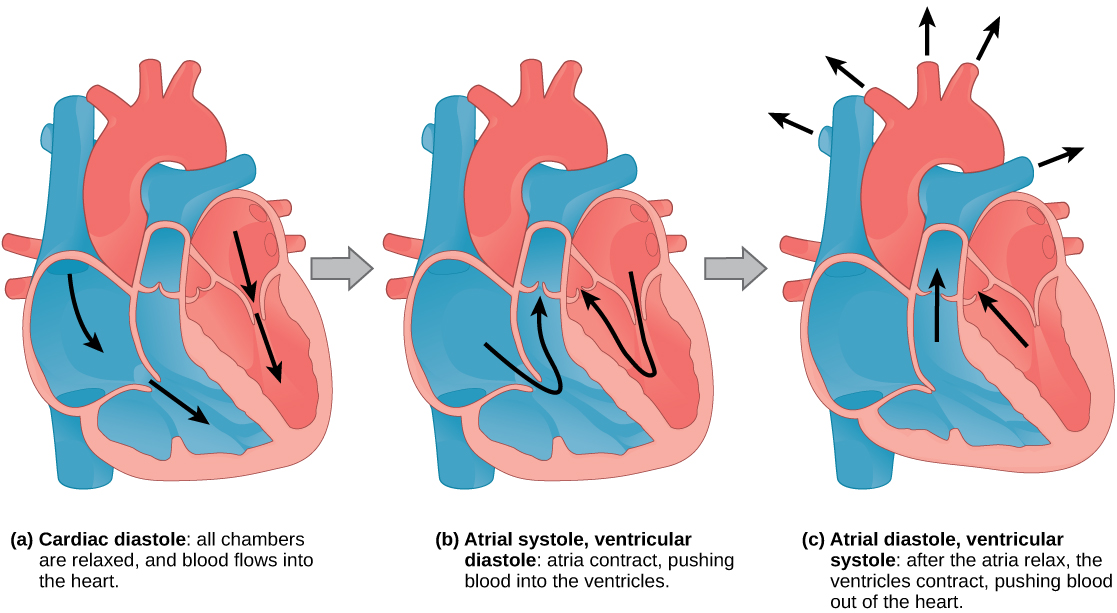
\includegraphics[width=14cm]{heart.jpg}
\centering
\caption{Heart contractions during a cardiac cycle}
\end{figure}
\

Mechanical vibrations reflect the turbulence that occurs when heart valves close. Traditionally, a stethoscope is used in cardiac auscultation to listen to these sounds that provide important acoustic information regarding the health condition of the heart. 
\\

Phonocardiography, is a diagnostic technique that creates a graphic record, called phonocardiogram, of the sounds and murmurs produced by the contracting heart. The phonocardiogram is obtained either with a chest microphone or with a miniature sensor in a small tubular instrument that is introduced through the blood vessels into one of the heart chambers. The phonocardiogram usually supplements the information obtained by listening to body sounds with a stethoscope (auscultation) and is of special diagnostic value when performed simultaneously with measurement of the electrical properties of the heart (electrocardiography) and pulse rate.
\\

The time-frequency analysis of the PCG signals permits detecting and characterising abnormal murmurs or extra sounds (systole or diastole) in the diagnosis of heart disease. In this study, we analyse normal, murmur and extra heart sounds recordings, separating them from artifacts. Most often, the symptoms of cardiovascular diseases become worse over time and detecting them with noninvasive techinques in early stages is crucial.
\\

The corelation among the phonocardiogram and the biological phenomenom is presented in the following diagram:

\begin{figure}[h]
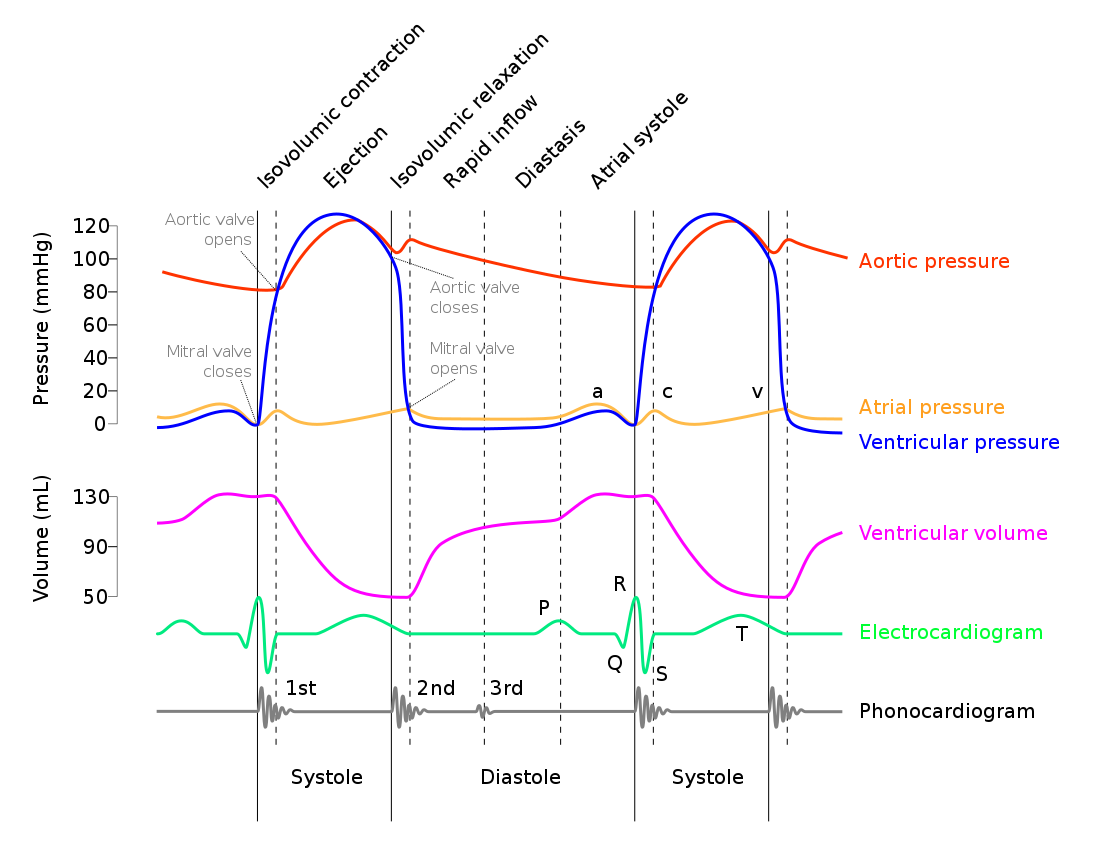
\includegraphics[width=15cm]{Wiggers_Diagram_2.png}
\centering
\caption{The Wiggers Diagram illustrating the cardiac cycle}
\end{figure}
\
\\
\
\\
\
\\
\
\\
\

\textbf{Heart murmur}
\\

Heart murmurs are heart sounds produced when blood flows across one of the heart valves that are loud enough to be heard with a stethoscope. Heart murmurs are most frequently categorized, into systolic murmurs and diastolic murmurs, differing in the part of the heartbeat on which they can be heard. There are also, continuous murmurs cannot be directly placed into either category.
\\

Systolic murmurs are due to blood flow through the semilunar valves. They occur at the start of blood ejection — which starts after S1 — and ends with the cessation of the blood flow — which is before S2. Diastolic murmurs start after S2 and end before S1. Many involve stenosis of the atrioventricular valves or regurgitation of the semilunar valves.
\\
\
\\

\textbf{Heart arrhythmia and extra beats}
\\

Heart arrhythmia (also known irregular heartbeat) is a group of conditions in which the heartbeat is irregular, too fast, or too slow. There are four main types of arrhythmia: extra beats, supraventricular tachycardias, ventricular arrhythmias, and bradyarrhythmias. Extra beats, part of our dataset, come in two different types, premature atrial contractions and premature ventricular contractions. Often they cause no symptoms but may present with fluttering in the chest or a skipped beat.
\\


\addcontentsline{toc}{section}{I.2. Previous work}
\section*{II.2. Previous work}
\

Many studies have been done on phonocardiogram signal so far. The research on this topic increased nowadays due to improvement in signal processing techniques and new methods in big data analysis. A summary of the most important results obtained with the Classifying Heart Sounds PASCAL Challenge dataset can be found here [].
\\

The Classifying Heart Sounds Workshop 2012 is the first international workshop to focus on the use of statistical machine learning techniques to segment and classify real-world heart audio. The clallange for this workshop was to create a first level of screening of cardiac pathologies both in a Hospital environment by a doctor (using a digital stethoscope) and at home by the patient (using a mobile device). 
\\

The problem is of particular interest to machine learning researchers as it involves classification of audio sample data, where distinguishing between classes of interest is non-trivial. Success in classifying this form of data requires extremely robust classifiers. 
\\

\begin{figure}[h]
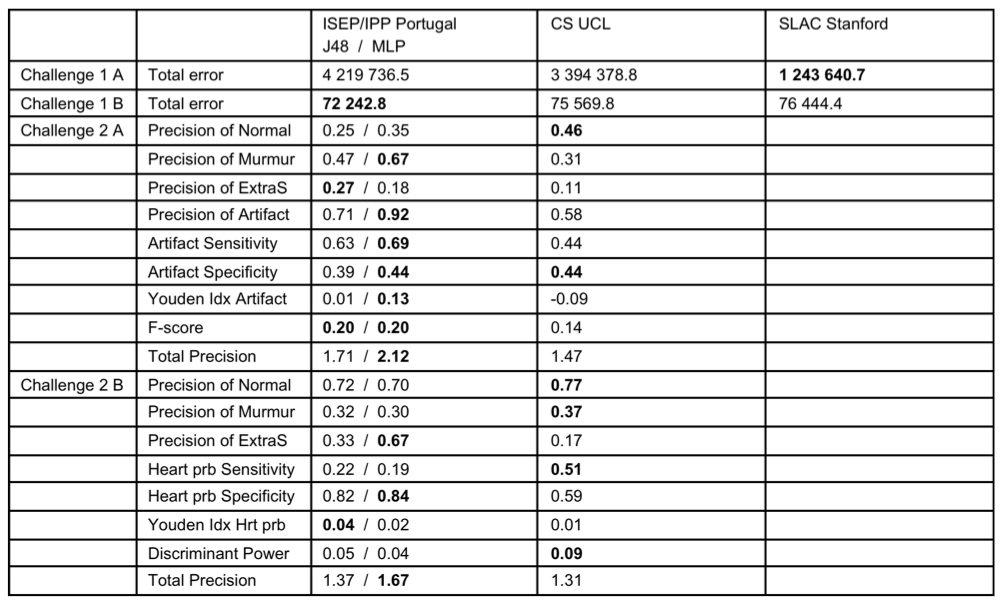
\includegraphics[width=16cm]{challengeresults.png}
\centering
\caption{A summary of the results of the three finalists from their approaches}
\end{figure}

The first team uses, after the segmentation, the J48 and MLP algorithms (using Weka) to train and classify the computed features. The UCL team exploits domain knowledge and compares the features of heartbeat before and after dropping out extra peaks and the smallest interval. By doing so they try to minimize the negative effect of noise. In the literature there are other proposed ways to tackle this challenge: partial least squares regression, neural networks and convolution neural networks.
\\

Other models for classifing the heart sounds can be found [kaggle], where the best general accuracy obtained was $93,18 \%$ for all the classes. The model proposed is a neural network.


\newpage



\addcontentsline{toc}{chapter}{II. Methodology and research methods}
\chapter*{II. Methodology and research methods}

\addcontentsline{toc}{section}{II.1. CRISP-DM Methodology}
\section*{II.1. CRISP-DM Methodology}
\

Cross-industry standard process for data mining, commonly known by its acronym CRISP-DM, is a data mining process model that describes commonly used approaches used to tackle problems. The current process model for data mining provides an overview of the life cycle of a data mining project. It contains the phases of a project, their respective tasks, and the relationships between these tasks. At this level, it is not possible to identify all relationships. Relationships could exist between any data mining tasks depending on the goals, the background, the interest of the user and on the data. 
\\

The life cycle of a data mining project consists of six phases, shown in the next figure. The sequence of the phases is not fixed. Moving back and forth between different phases can be required. The outcome of each phase determines which phase has to be performed next. The arrows indicate the most important and frequent dependencies between phases.
\\

\begin{figure}[h]
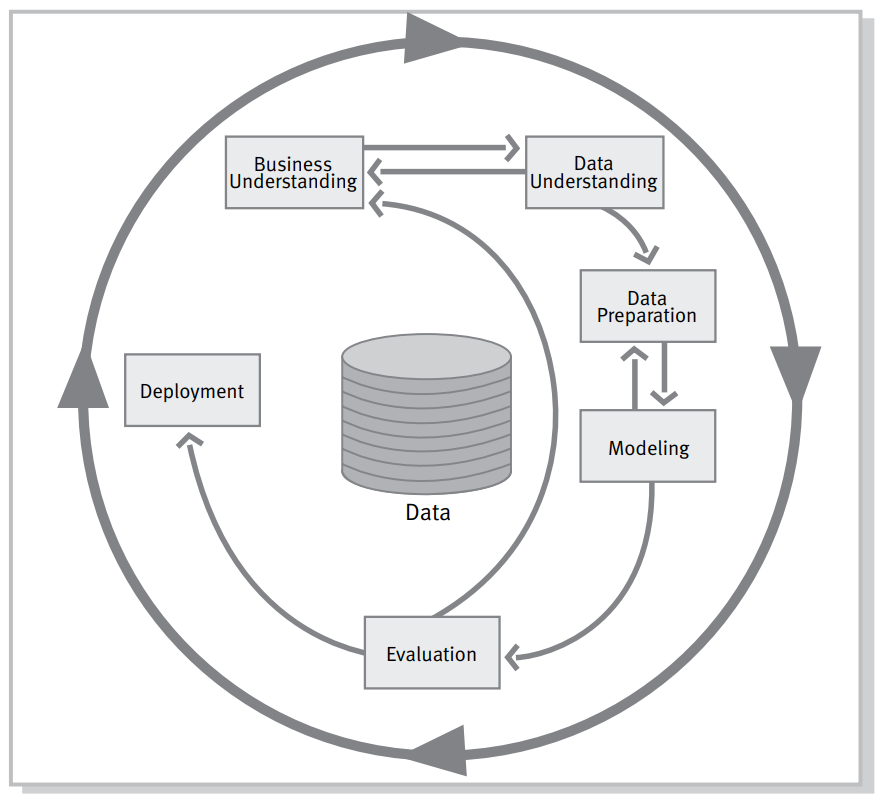
\includegraphics[width=8cm]{crisp.png}
\centering
\caption{Phases of the CRISP-DM model}
\end{figure}
\


\textbf{Business understanding}

\

The initial phase main purpose is understanding the project objectives and requirements from a business perspective, analysing the available resources, and then converting this knowledge into a data mining problem definition, and a plan designed to achieve all the objectives. 
\\

For our study the main objective is to predict with a high rate of trust if a person has arrhythmia or murmurs through a phonocardiogram. The resources available for us are a dataset of different types of recordings, a graphic card GeForce GTX 1050 (2GB) and a Intel(R) Core(TM) i7-7700HQ CPU @ 2.80GHz. Our initial goal would be to get a minimum of 70\% accuracy.
\\

\textbf{Data understanding}

\

The data understanding phase starts with an initial data collection and proceeds with activities that can give insides about the data, to identify data quality problems, or to detect interesting subsets to form hypotheses for hidden information.
\\

Our dataset has been gathered from two sources. All the files are .wav files with lengths between 1 second and 30 seconds and two frequencies: 44100 Hz and 4000 Hz. We also have examples of recordings thare are not heartbeats, but artifacts.
\\

\textbf{Data preparation}

\

This phase covers all activities to construct the final dataset (data that will be used for creating the model) from the initial raw data. Tasks representative for the data preparation phase include table, record, and attribute selection as well as transformation and cleaning of data for modeling tools.
\\

In this phase we normalised each recording using the Frobenius norm and after this, using a peak detection algorithm, we identfied the sounds S1 and S2 in each recording. We searched for the peaks starting with second 0,5 and ended at len(rec) - 0,5 seconds. For each peak we chunked a 1 second peice of the record, obtaining multiple one second recordings. In order to get a better accuracy through multiplying the data we used a sliding window technique.
\\

\textbf{Modeling}

\

In this phase, various modeling techniques are selected and applied, and their parameters are calibrated to optimal values. Usualy, there are several techniques for the same data mining problem type. Some techniques have specific requirements on the form of data.
\\

The models we created are one Convolutional Neural Networks that classifies each record in one of the four classes, and the second model uses a Multi-Task Learning technique in Convolutional Neural Networks.

\textbf{Evaluation}

\

At this stage in the project you have built a model (or models) that appears to have good quality, from a data analysis perspective. Before proceeding to final deployment of the model, it is important to evaluate the model, and review the steps executed to construct the model, to be certain it achieves the business objectives.
\\

The metrics we used for evaluating the models is te accuracy of the test dataset. Other metrics that we used are the validation dataset accuracy, the value of the loss function, the sensitivity and the specificity.
\\

\textbf{Deployment}

\

Creation of the model is not the end of the project. Even if the purpose of the model is to increase knowledge of the data, the knowledge gained will need to be organized and presented in a way that is useful to the users. Depending on the requirements, the deployment phase can be as simple as generating a report or as complex as implementing an application from scratch. In many cases it will be the customer who will carry out the deployment steps. 



\begin{figure}[h]
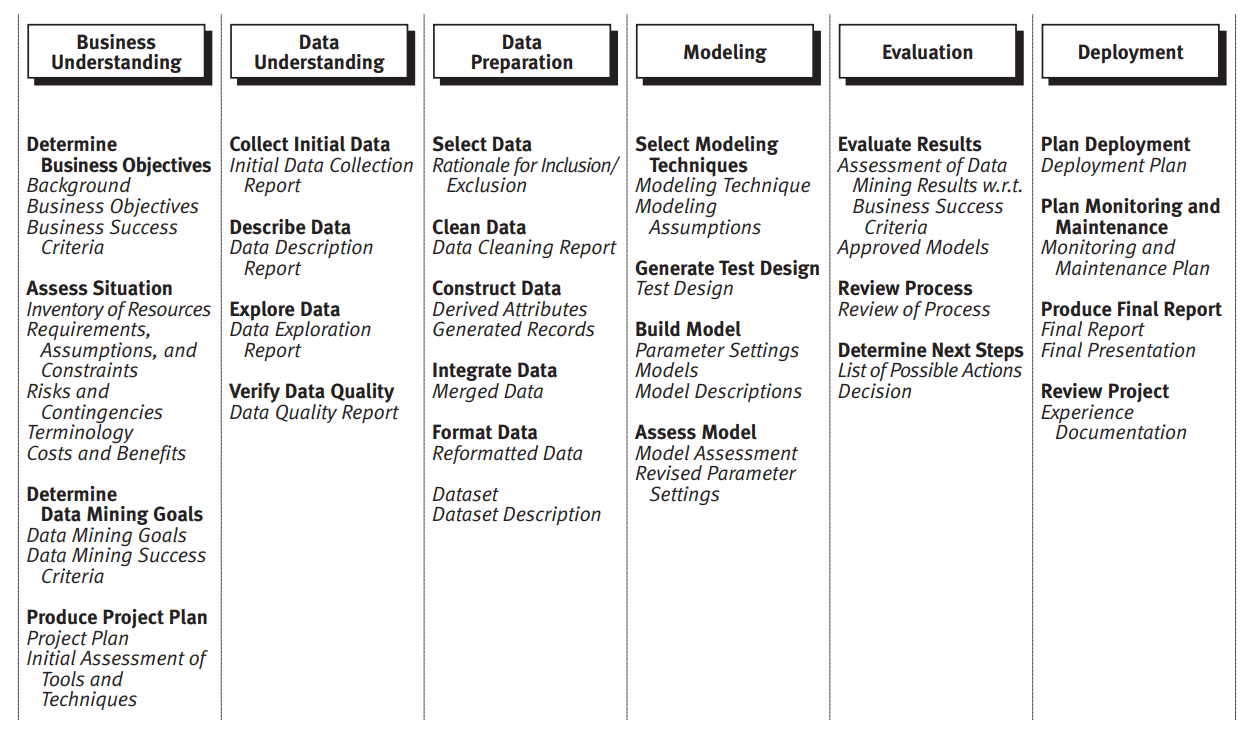
\includegraphics[width=16.2cm]{crispt.png}
\centering
\caption{Generic tasks and outputs of the CRISP-DM model}
\end{figure}
\

In the next sections we will detaliate some of the most important and time consuming phases of the project, detaliating the mathemathical and biological backgroung for each stage.
\

\addcontentsline{toc}{section}{II.2. Data understanding and preparation}
\section*{II.2. Data understanding and preparation}

\

\addcontentsline{toc}{subsection}{II.2.1. Data Description and Organisation}
\subsection*{II.2.1. Data Description and Organisation}

\

The dataset is split into two sources, A and B. The recordings from the A dataset are gathered from the general public via the iStethoscope Pro iPhone app. The second dataset, B, is collected from a clinic trial in hospitals using the digital stethoscope DigiScope. Most information in heart sounds is contained in the low frequency components, with noise in the higher frequencies.
\\

The audio files have varying lengths, between 1 second and 30 seconds (some have been clipped to reduce excessive noise and provide the salient fragment of the sound). The two datasets differ in number, frequency and other proprieties of the .wav files.
\\

\textbf{Dataset A}

\

The recordings from this dataset are gathered using the iStethoscope Pro iPhone app. All of them are represented with on a 705  bitrate, throuhg a mono channel. The samples rate is 44100 Hz. The following types of heartbeats are recorded and labeled:

\

Atraining\_normal 14Mb 31 files
\

Atraining\_murmur 17.3Mb 34 files
\

Atraining\_extrahs 6.9Mb 19 files
\

Atraining\_artifact 22.5Mb 40 files

\

\textbf{Dataset B}

\

The recordings from this dataset are gathered using the iStethoscope Pro iPhone app. All of them are represented with on a 705  bitrate, throuhg a mono channel. The samples rate is 44100 Hz. The following types of heartbeats are recorded and labeled:

\

Btraining\_normal 13.8Mb 320 files
\

Btraining\_murmur 5.3Mb 95 files
\

Btraining\_extrasystole 1.9Mb 46 files
\


\addcontentsline{toc}{subsection}{II.2.2. Data}
\subsection*{II.2.2. Data}

\

\addcontentsline{toc}{section}{II.3. Modeling}
\section*{II.3. Modeling}

\

\addcontentsline{toc}{section}{II.4. Technologies}
\section*{II.4. Technologies}

\

\newpage

\addcontentsline{toc}{chapter}{III. Results}
\chapter*{III. Results}

\

Criptografia a apărut pe vremea egiptenilor, cu peste 4000 de ani în urmă. În principal, până la începutul secolului al XX-lea, criptografia s-a ocupat mai ales de şabloane lingvistice. De atunci, accentul s-a mutat pe folosirea extensivă a matematicii, inclusiv a aspectelor de teoria informaţiei, complexitatea algoritmilor, statistică, combinatorică, algebră abstractă şi teoria numerelor. Din punct de vedere lexicografic, cuvântul \textit{criptografie} este format din rădăcinile \textit{cryptos} şi \textit{grafie}.

\begin{center}
Criptografie = \textit{cryptos}(ascuns) + \textit{grafie}(a scrie)
\end{center}
\

Criptografia este o componentă a domeniului securităţii informaţiei şi poate fi definită astfel:

\begin{definition} \textit{Criprografia} este studiul tehnicilor matematice care se ocupă de următoarele aspecte ale securităţii informaţiei: confidenţialitatea, autentificarea, non-repudierea mesajelor şi integritatea datelor.
\end{definition}
\

Principalele obiective ale unui sistem criptografic sunt:
\begin{itemize}
	\item \textit{Confidenţialitatea}: proprietatea de a păstra secretul informaţiei, astfel încât aceasta să fie utilizată numai de către persoane autorizate.
	\item \textit{Autentificarea}: proprietatea de a identifica o entitate conform anumitor standarde. Aceasta implică:		
	\begin{enumerate}
		\item Autentificarea unei entităţi;
		\item Autentificarea sursei informaţiei.
	\end{enumerate}
	\item \textit{Non-repudierea}: proprietatea care previne negarea unor evenimente anterioare.
	\item \textit{Integritatea datelor}: proprietatea de a evita orice modificare (inserare, ştergere, substituţie) neautorizată a informaţiei.
\
\end{itemize}


\newpage

\addcontentsline{toc}{chapter}{IV. Conclusion}
\chapter*{IV. Conclusion}

\nocite{*}
\addcontentsline{toc}{chapter}{VI. Bibliography}
\bibliographystyle{plain}
\bibliography{bibliografie}

%% F6 F11 F6 F6 Quick Build

\end{document}